\chapter{Vector}

\section{Three Dimensional Coordinate System}

\begin{formula}[Distance Formula in 3D]
  The distance \(|P_1P_2|\) between the points \(P_1(x_1, y_1, z_1)\) and \(P_2(x_2, y_2, z_2)\) is
  \[
    |P_1P_2| = \sqrt{(x_2 - x_1)^2 + (y_2 - y_1)^2 + (z_2 - z_1)^2}
  \]
\end{formula}

\begin{formula}[Equation of a Sphere]
  The equation of a sphere with center \(C(h, k, l)\) and radius \(r\) is
  \[
    (x - h)^2 + (y - k)^2 + (z - l)^2 = r^2
  \]
  In particular, if the center is the origin \(O\), then an equation of the sphere is
  \[
    x^2 + y^2 + z^2 = r^2
  \]
\end{formula}

\section{Vectors}

\textbf{Figure: }Triangle Law of Vector Addition

\begin{figure}[!h]
  \centering
  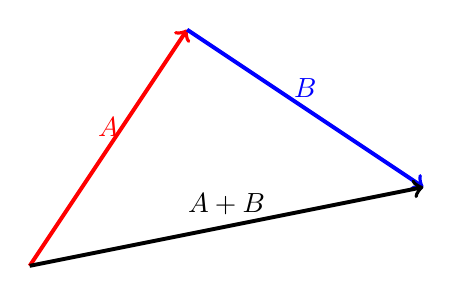
\begin{tikzpicture}
    \centering
    \draw[->, line width=0.5mm, red] (0, 0) -- (2, 3) node[midway, above] {\(A\)};
    \draw[->, line width=0.5mm, blue] (2, 3) -- (5, 1) node[midway, above] {\(B\)};
    \draw[->, line width=0.5mm, black] (0, 0) -- (5, 1) node[midway, above] {\(A + B\)};
  \end{tikzpicture}
\end{figure}

\begin{formula}[Vector Subtraction]
  The vector \(A - B\) is defined as
  \[
    A - B = A + (-B)
  \]
\end{formula}

\textbf{Figure: }Vector Subtraction

\begin{figure}[!h]
  \centering
  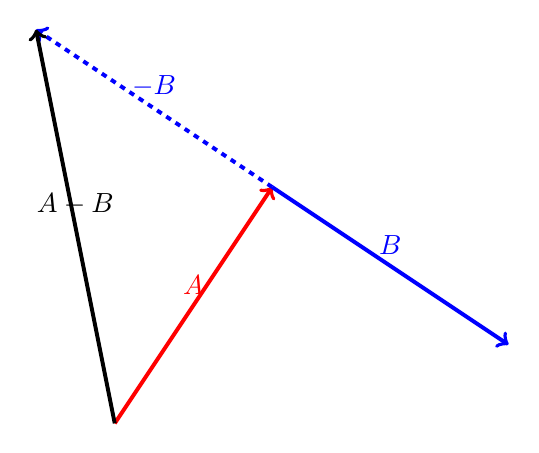
\begin{tikzpicture}
    \centering
    \draw[->, line width=0.5mm, red] (0, 0) -- (2, 3) node[midway, above] {\(A\)};
    \draw[->, line width=0.5mm, blue] (2, 3) -- (5, 1) node[midway, above] {\(B\)};
    \draw[->, dash pattern=on 2pt off 2pt, line width=0.5mm, blue] (2, 3) -- (-1, 5) node[midway, above] {\(-B\)};
    \draw[->, line width=0.5mm, black] (0, 0) -- (-1, 5) node[midway, above] {\(A - B\)};
  \end{tikzpicture}
\end{figure}

\section{Components of a Vector}

\begin{figure}[!h]
  \centering
  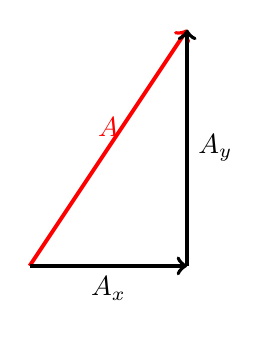
\begin{tikzpicture}
    \centering
    \draw[->, line width=0.5mm, red] (0, 0) -- (2, 3) node[midway, above] {\(A\)};
    \draw[->, line width=0.5mm, black] (0, 0) -- (2, 0) node[midway, below] {\(A_x\)};
    \draw[->, line width=0.5mm, black] (2, 0) -- (2, 3) node[midway, right] {\(A_y\)};
  \end{tikzpicture}
\end{figure}